\section{Integrations}
Spring XD integration modules are Message Endpoints \cite{enterprise-inetgration-pattern} that responsible for sending to and receiving data from external agents.  There are 3 types of message endpoints: Source, Sinks and Batch Jobs.  The source's responsibility is to receive the inbound data and convert it to a message that will be used by modules in the stream(reference streams) or by a job that is launched based on the receipt of the data.  The sink's responsibility is to convert the message to the format that can be consumed by the external agent and transmit the data to the agent.   Batch Jobs may be used to execute specialized logic on a large set of data from one external agent and transmit the resulting data to another external agent.  Spring XD offers a suite of 23 sources (file, jdbc, Mongo, HDFS, \ldots), 24 sinks (file, jdbc, Mongo, HDFS, \ldots) and 9 jobs (filepollhdfs, sparkapp, sqoop, \ldots)  that are ready to use at XD startup.  
If an existing module does meet the needs of for the given use case a user may create a custom integration module.\par
A source's responsibility is to receive the inbound data and convert it to a message for use by modules in a stream or by a batch job.  There are 2 types of source: Poller and Socket.  A poller source will interrogate an external agent for data at a interval specified by the user.  A socket source will have a port open ready to receive data that is pushed from an external agent.  \par
 There are 2 types of sinks: Counter/gauge and Delegate.  A counter/gauge is a specialized sink increments a field on a datastore every time a message is received refer to the (Analytics Section) for more information.  As a delegate sink's responsibility is to translate the XD message to the format that can be used by the external agent and dispatch that data to the agent.  
	A batch job's responsibility is to read and or write of data from an external agent, execute a migration of data that needs transactional safeguards or to execute an external process (SparkApp). \par
Use Cases 
With the advent of microservices \cite{microservices-pattern} applications are becoming evermore integrated.  In cases where an agent needs access to microservices but does not have the capability to transmit the request via the API presented, or an agent needs to take the results of a microservice and transmit it to  an external agent in the agent's accepted format, XD can bridge that chasm. 
An example of this would be if we needed a service that would receive sensor data via mqtt and write that the data to hdfs. The following stream would be used to do this: "mqtt|hdfs".
Another example of this would be a scenario if a database is being updated by an service but while the database is updated we need to update a collection in a mongo collection with this data.  This can be done by creating a stream that would monitor a table(s) retrieve changes and write the results to the mongo collection.  This would be respresented by the following stream: "jdbc --fixedDelay=1 --split=1 --query='select * from testfoo where tag = 0' --update='update testfoo set tag=1 where fooid in (:fooid)'|log" \par
Example Source
jdbc - is a poller source that will execute a query against a database and generate a message for each row that is retrieved.  \cite{jdbc-module}
mqtt - is a socket source that awaits for mqtt messages to be received once the message is received the payload of the message is sent as an XD message to the next module in the stream.  \cite{mqtt-module}
Example Sink
Mongo - The Mongo sink writes messages into a Mongo collection \cite{mongo-module}
hdfs - writes messages to the specified location on a hadoop instance. \cite{hadoop-hdfs-module}
Example Job
filejdbc -A module which loads CSV files into a JDBC table

Integration Modules are deployed in the modules subdirectory and are segregated in subdirectories by type: modules/source, modules/sink and modules/job.  
These modules are dynamically loaded when a stream or job is created that requires that specific module.  Once loaded, they are stored in Java's classloader and will not be reloaded (until the XD container is restarted).  Besides the pre-existing integration modules that come with the XD installation a user may create their own integration modules. \par

Spring XD uses Spring Integration \cite{spring-integration-reference} as its foundation for implementing source, sink and batch modules.  As such integration modules are comprised minimally of one channel and a integration bean.  In the case of a source module there is an "output" channel to dispatch messages transmitted by the integration bean to the stream figure~\ref{fig:sourcembc}. 
\begin{figure}[ht]
\centering
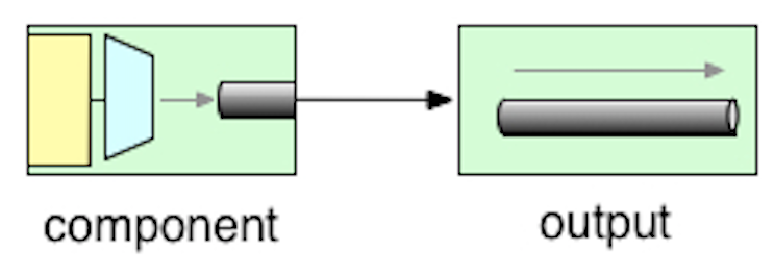
\epsfig{file=integration-module-output-channel.eps, height=.8in, width=2in}
\caption{Source Module Basic Components}
\label{fig:sourcembc}
\end{figure}

 For a sink there is an "input" stream for which all messages from the stream will be dispatched and then read by the integration bean figure~\ref{fig:sinkmbc}. 

\begin{figure}
\centering
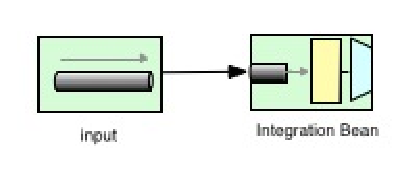
\epsfig{file=integration-module-input-channel.eps, height=.8in, width=2in}
\caption{Sink Module Basic Components}
\label{fig:sinkmbc}
\end{figure}

Current end. \par